\PassOptionsToPackage{unicode}{hyperref}
\documentclass[aspectratio=1609, professionalfonts, 9pt, bibliography=totoc]{beamer}

\usefonttheme[onlymath]{serif}
\usetheme[showtotalframes]{tudo}

\usepackage{polyglossia}
\setmainlanguage{german}
\usepackage[style=alphabetic]{biblatex}
\addbibresource{lit.bib}

% Mathematik
\usepackage{amsmath}
\usepackage{amssymb}
\usepackage{mathtools}
\usepackage{cancel}

\usepackage{hyperref}
\usepackage{bookmark}

%%%%%%%%%%%%%%%%%%%%%%%%%%%%%%%%%%%%%%%%%%%%%%%%%%%%%%%%%%%%%%%%%%%%%%%%%%%%%%%%
%%%%%-------------Hier Titel/Autor/Grafik/Lehrstuhl eintragen--------------%%%%%
%%%%%%%%%%%%%%%%%%%%%%%%%%%%%%%%%%%%%%%%%%%%%%%%%%%%%%%%%%%%%%%%%%%%%%%%%%%%%%%%

%Titel:
\title{Global Positioning System}
%Autor
\author[C.~Beckmann]{Christian Beckmann}
%Lehrstuhl/Fakultät
\institute[Seminar Physik des Segelns]{Physik des Segelns \\ Seminar}
%Titelgrafik
\titlegraphic{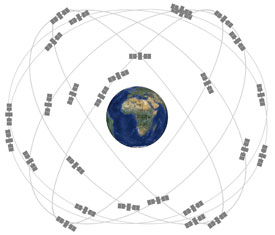
\includegraphics[width=0.3\textwidth]{images/constellation.jpg}}


\begin{document}

\maketitle

\begin{frame}
    \frametitle{Einführung}
    \tableofcontents[pausesections]
\end{frame}

\section{Grundlagen}
\begin{frame}
	\frametitle{Grundlagen}
    \begin{block}{Betreiber}
        US-Regierung, Verteidigungsministerium
    \end{block}
    \begin{block}{Budget}
        2017: \$908,262 mil.\\
        2018: \$1,1 mrd
    \end{block}
    Bezahlt aus den Steuern der US-Bürger
    \cite{gpsgov}
\end{frame}

%\begin{frame}{Historische Meilensteine}
%    \begin{columns}
%        \begin{column}{0.5\paperwidth}
%            \begin{itemize}
%                \item 1957: Sputnik
%                \item 1964: US-Marine, TRANSIT System
%                \begin{itemize}
%                    \item Bill Guier (Mathematiker)
%                    \item George Weiffenbach (Physiker)
%                \end{itemize}
%            \end{itemize}
%        \end{column}
%        \begin{column}{0.5\paperwidth}
%            \begin{figure}
%                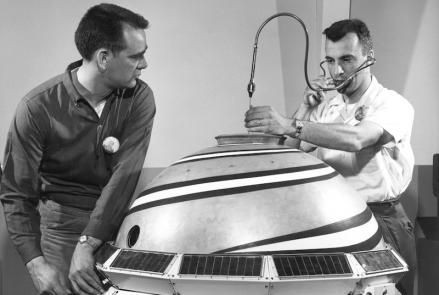
\includegraphics[width=0.4\paperwidth]{images/transit-satellite.jpg}
%                \caption{Tests am zweiten Transit Satelliten, }%\cite{TimeAndNavigation}}
%                \label{fig:transit}
%            \end{figure}
%        \end{column}
%    \end{columns}
%\end{frame}

\section{Literatur}
\begin{frame}{Literatur}
    \printbibliography
\end{frame}
